\documentclass[a4paper,10pt]{article}
\usepackage[utf8]{inputenc}
\usepackage{ngerman}
\usepackage{eurosym}
\usepackage{algorithm2e}
%\usepackage{ stmaryrd }
\usepackage{enumerate}
\usepackage{tikz}
\usetikzlibrary{trees,automata,arrows,shapes}
\usepackage{graphicx}
\usepackage{listings}
\usepackage{xcolor}
\usepackage{amsmath, amsthm}
\usepackage{listings}
\usepackage{amsfonts, amssymb}
\usepackage{algorithm2e}
\usepackage{textcomp}
\usepackage{bussproofs}
\usepackage{rotating}
\usepackage{caption}
\usepackage{listings}% http://ctan.org/pkg/listings
\lstset{
  basicstyle=\ttfamily,
  mathescape
}
\renewcommand*{\proofname}{Beweis}

%opening
\title{}
\author{}

\begin{document}
\noindent Thomas Stüber (3750920) \hfill Tübingen, den  \today\\
\noindent Benjamin Coban (3526251) \\
\begin{center}
\Large Übungen zur Vorlesung  \\ ``SAT-Solving und Anwendungen'' \\
\vspace*{2mm}
\large (Abgabe 10) \\
\vspace*{2mm}
\end{center}

\noindent\textbf{Aufgabe 10.1}\\
CDCL Algorithmus anzuwenden.\\\\
\begin{center}
	\begin{tabular}{|c|c|c|c|c|}
		\hline 
		Level & Variable & Value & Reason & Clause \\ 
		\hline 
		1 & x & T & Decision &  \\ 
		\hline 
		2 & y & T & Decision &  \\ 
		\hline 
		& z & T & R & $\{ \neg x,\neg y, z\}$ \\ 
	 
		\hline 
		3 & u & T & Decision &  \\ 
		\hline 
		& v & F & R & $\{ \neg t,\neg u,\neg v\}$ \\ 
		\hline
		& w & F & R & $\{ \neg x,\neg y,\neg z,\neg w\}$ \\ 
		\hline 
		& p & T & R & $\{ \neg u, v,p,\neg y,\neg x\}$ \\ 
		\hline 
		& p  & F & R & $\{ w,\neg p, \neg z, v\}$ \\ 
		\hline 
	\end{tabular} 
\end{center}
Aus der Tabelle entsteht folgender Implikationsgraph, wobei die Knoten die Variablen enthalten. Die Level sind zeilenweise zu lesen, eine Kante ist eingetragen, wenn die Klausel die Variable des Startknotens enthält. 
\begin{center}
	\begin{center}
		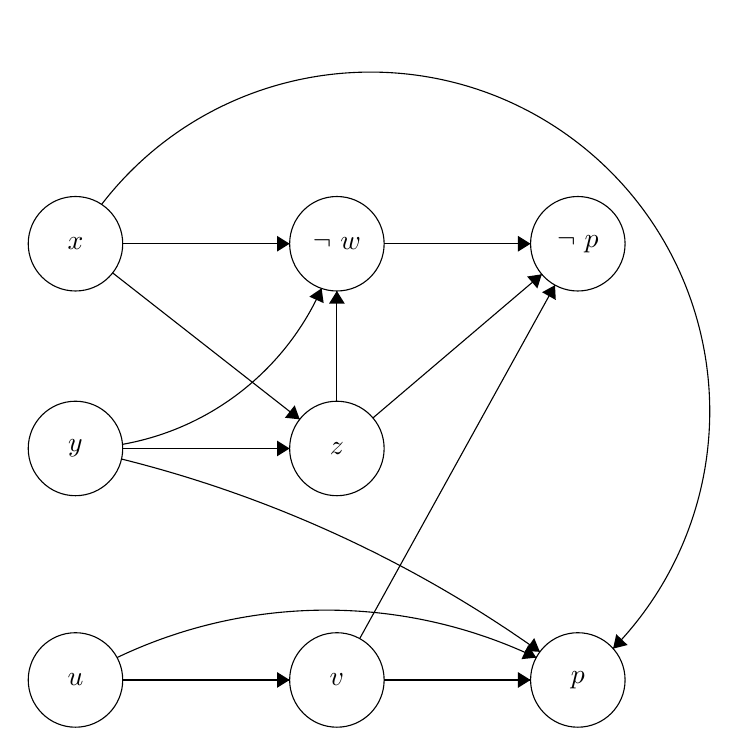
\begin{tikzpicture}[scale=0.2]
		\tikzstyle{every node}+=[inner sep=0pt]
		\draw [black] (15.2,-14.2) circle (3);
		\draw (15.2,-14.2) node {$x$};
		\draw [black] (15.2,-27.2) circle (3);
		\draw (15.2,-27.2) node {$y$};
		\draw [black] (15.2,-41.9) circle (3);
		\draw (15.2,-41.9) node {$u$};
		\draw [black] (31.8,-27.2) circle (3);
		\draw (31.8,-27.2) node {$z$};
		\draw [black] (31.8,-41.9) circle (3);
		\draw (31.8,-41.9) node {$v$};
		\draw [black] (47.1,-41.9) circle (3);
		\draw (47.1,-41.9) node {$p$};
		\draw [black] (31.8,-14.2) circle (3);
		\draw (31.8,-14.2) node {$\neg\mbox{ }w$};
		\draw [black] (47.1,-14.2) circle (3);
		\draw (47.1,-14.2) node {$\neg\mbox{ }p$};
		\draw [black] (18.2,-27.2) -- (28.8,-27.2);
		\fill [black] (28.8,-27.2) -- (28,-26.7) -- (28,-27.7);
		\draw [black] (17.56,-16.05) -- (29.44,-25.35);
		\fill [black] (29.44,-25.35) -- (29.12,-24.46) -- (28.5,-25.25);
		\draw [black] (31.8,-24.2) -- (31.8,-17.2);
		\fill [black] (31.8,-17.2) -- (31.3,-18) -- (32.3,-18);
		\draw [black] (18.2,-14.2) -- (28.8,-14.2);
		\fill [black] (28.8,-14.2) -- (28,-13.7) -- (28,-14.7);
		\draw [black] (30.83,-17.035) arc (-23.9119:-79.9568:17.094);
		\fill [black] (30.83,-17.03) -- (30.05,-17.56) -- (30.96,-17.97);
		\draw [black] (18.2,-41.9) -- (28.8,-41.9);
		\fill [black] (28.8,-41.9) -- (28,-41.4) -- (28,-42.4);
		\draw [black] (34.8,-41.9) -- (44.1,-41.9);
		\fill [black] (44.1,-41.9) -- (43.3,-41.4) -- (43.3,-42.4);
		\draw [black] (17.84,-40.478) arc (115.5192:64.4808:30.894);
		\fill [black] (44.46,-40.48) -- (43.95,-39.68) -- (43.52,-40.58);
		\draw [black] (18.124,-27.87) arc (75.99165:54.52642:78.538);
		\fill [black] (44.69,-40.11) -- (44.33,-39.24) -- (43.75,-40.06);
		\draw [black] (16.859,-11.703) arc (142.41243:-44.35052:21.546);
		\fill [black] (49.34,-39.91) -- (50.26,-39.68) -- (49.54,-38.99);
		\draw [black] (34.8,-14.2) -- (44.1,-14.2);
		\fill [black] (44.1,-14.2) -- (43.3,-13.7) -- (43.3,-14.7);
		\draw [black] (33.25,-39.27) -- (45.65,-16.83);
		\fill [black] (45.65,-16.83) -- (44.83,-17.28) -- (45.7,-17.77);
		\draw [black] (34.09,-25.26) -- (44.81,-16.14);
		\fill [black] (44.81,-16.14) -- (43.88,-16.28) -- (44.53,-17.04);
		\end{tikzpicture}
	\end{center}
\end{center}
Die Reason Clause ist $\{\neg u, v,p,\neg y,\neg x\}$, die Conflict Clause $\{w,\neg p,\neg z,v\}$.
\newpage
\noindent\textbf{Aufgabe 10.2}\\
CDCL Algorithmus anzuwenden.
\begin{center}
	\begin{tabular}{|c|c|c|c|c|}
		\hline 
		Level & Variable  & Value & Reason & Clause \\ 
		\hline 
		1 & w & F & Decision &  \\
		\hline 
		2 & x & F & Decision &  \\ 
		\hline 
		& y & T & Reason & $\{x,y \}$ \\ 
		\hline 
		& z & T & Reason & $\{z,\neg y, x \}$ \\ 
		
		\hline 
		& a & T & R & $\{w,a\}$ \\ \hline  
		& a & F & Reason & $\{\neg a,\neg y,\neg z \}$ \\ 
		\hline 
	\end{tabular} 
\end{center}
Es entsteht folgender Implikationsgraph:
\begin{center}
	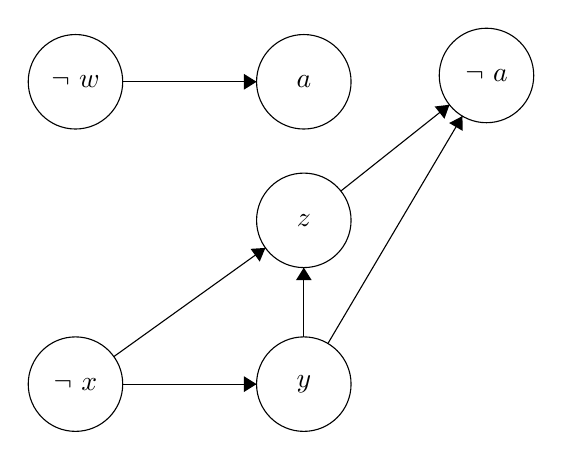
\begin{tikzpicture}[scale=0.2]
\tikzstyle{every node}+=[inner sep=0pt]
\draw [black] (17.2,-35) circle (3);
\draw (17.2,-35) node {$\neg\mbox{ }x$};
\draw [black] (17.2,-15.8) circle (3);
\draw (17.2,-15.8) node {$\neg\mbox{ }w$};
\draw [black] (31.7,-15.8) circle (3);
\draw (31.7,-15.8) node {$a$};
\draw [black] (31.7,-35) circle (3);
\draw (31.7,-35) node {$y$};
\draw [black] (31.7,-24.6) circle (3);
\draw (31.7,-24.6) node {$z$};
\draw [black] (43.3,-15.4) circle (3);
\draw (43.3,-15.4) node {$\neg\mbox{ }a$};
\draw [black] (20.2,-15.8) -- (28.7,-15.8);
\fill [black] (28.7,-15.8) -- (27.9,-15.3) -- (27.9,-16.3);
\draw [black] (20.2,-35) -- (28.7,-35);
\fill [black] (28.7,-35) -- (27.9,-34.5) -- (27.9,-35.5);
\draw [black] (31.7,-32) -- (31.7,-27.6);
\fill [black] (31.7,-27.6) -- (31.2,-28.4) -- (32.2,-28.4);
\draw [black] (19.64,-33.25) -- (29.26,-26.35);
\fill [black] (29.26,-26.35) -- (28.32,-26.41) -- (28.9,-27.22);
\draw [black] (33.23,-32.42) -- (41.77,-17.98);
\fill [black] (41.77,-17.98) -- (40.93,-18.42) -- (41.79,-18.92);
\draw [black] (34.05,-22.74) -- (40.95,-17.26);
\fill [black] (40.95,-17.26) -- (40.01,-17.37) -- (40.63,-18.15);
\end{tikzpicture}
\end{center}
\end{document}
